        %%******************************************%%
        %%                                          %%
        %%        Modello di tesi di laurea         %%
        %%            di Andrea Giraldin            %%
        %%                                          %%
        %%             2 novembre 2012              %%
        %%                                          %%
        %%******************************************%%

\begin{document}
    \frontmatter
    \begin{titlepage}
    \begin{center}
        \begin{LARGE}
            \textbf{\myUni}\\
        \end{LARGE}

        \vspace{10pt}

        \begin{Large}
            \textsc{\myDepartment}\\
        \end{Large}

        \vspace{10pt}

        \begin{large}
            \textsc{\myFaculty}\\
        \end{large}

        \vspace{30pt}
        \begin{figure}[htbp]
            \centering
            
\includegraphics[height=6cm]{unipd-logo}
        \end{figure}
        \vspace{30pt}

        \begin{LARGE}
            \textbf{\myTitle}\\
        \end{LARGE}

        \vspace{10pt}

        \begin{large}
            \textsl{\myDegree}\\
        \end{large}

        \vspace{40pt}

        \begin{large}
            \begin{flushleft}
                \textit{Relatore}\\
                \vspace{5pt}
                \profTitle\ \myProf
            \end{flushleft}

            % You can tweak the spacing to have professor and student names on the same line
            % useful if the page is broken by a long thesis title and you need more space
            % \vspace{-52pt}

            \begin{flushright}
                \textit{Laureando}\\
                \vspace{5pt}
                \myName
                \space
                \myMatr
            \end{flushright}
        \end{large}

        \vspace{40pt}

        \line(1, 0){338} \\
        \begin{normalsize}
            \textsc{Anno Accademico \myAA}
        \end{normalsize}
    \end{center}
\end{titlepage}

    \clearpage
\phantomsection
\thispagestyle{empty}

\hfill
\vfill

\noindent\myName: \textit{\myTitle,}
\myDegree,
\textcopyright\ \myTime.

    \cleardoublepage
\phantomsection
\thispagestyle{empty}
\pdfbookmark{Dedica}{Dedica}

\vspace*{3cm}

\begin{center}
    Lorem ipsum dolor sit amet, consectetuer adipiscing elit. \\ \medskip
    --- Oscar Wilde
\end{center}

\medskip

\begin{center}
    Dedicato a ...
\end{center}

    \cleardoublepage
\phantomsection
\pdfbookmark{Sommario}{Sommario}
\begingroup
\let\clearpage\relax
\let\cleardoublepage\relax
\let\cleardoublepage\relax

\chapter*{Sommario}

Il seguente documento ha lo scopo di descrivere in modo dettagliato il lavoro svolto durante il periodo di stage, dal laureando Andrea Meneghello, della durata di trecentododici ore, presso l'azienda THRON S.p.A.
L'obiettivo principale del progetto di stage è stato realizzare un portale per favorire la consultazione delle API pubbliche e private di THRON, attraverso una soluzione centralizzata.\\
Il portale è stato sviluppato utilizzando il framework Vue.js accompagnato da vari strumenti del suo ecosistema, ed è stato protetto con autenticazione seguendo lo standard Oauth2, integrandosi con il provider aziendale Azure.
Oltre alla consultazione della documentazione, il portale deve permettere all'utente di provare le API direttamente dall'interfaccia in modo intuitivo, permettendo inoltre il download delle stesse in formato yaml.\\
Infine tutte le componenti implementate sono state opportunatamente documentate e il loro corretto funzionamento è stato verificato tramite test di unità e di accettazione.

%\vfill

%\selectlanguage{english}
%\pdfbookmark{Abstract}{Abstract}
%\chapter*{Abstract}

%\selectlanguage{italian}

\endgroup

\vfill

    \cleardoublepage\phantomsection\pdfbookmark{Ringraziamenti}{ringraziamenti}

\begin{flushright}{
    \slshape
    ``The future belongs to those who believe in the beauty of their dreams.''} \\
    \medskip
    --- Eleanor Roosevelt
\end{flushright}


\bigskip

\begingroup
\let\clearpage\relax
\let\cleardoublepage\relax
\let\cleardoublepage\relax

\chapter*{Ringraziamenti}

\noindent \textit{Innanzitutto, desidero esprimere la mia profonda gratitudine alla Prof.ssa \myProf, relatrice della mia tesi, per la sua guida e sostegno durante la stesura di questa tesi. Senza il suo prezioso contributo, questo lavoro non sarebbe stato realizzabile.\\}

\noindent \textit{Vorrei ringraziare di cuore i miei genitori e la mia famiglia per il loro amore, la loro comprensione e il loro costante supporto incondizionato. Senza di voi questo percorso non sarebbe stato possibile.\\}

\noindent \textit{Alla mia fidanzata, desidero ringraziarti per la tua pazienza e per aver sempre creduto in me. Sei stata il mio sostegno morale che mi ha spinto a raggiungere questo traguardo. \\}

\noindent \textit{Infine vorrei ringraziare tutti i miei amici per essere stati sempre al mio fianco, per avermi incoraggiato nei momenti difficili e per aver condiviso cone me questa avventura accademica.\\}

% \noindent \textit{Innanzitutto, vorrei esprimere la mia gratitudine alla Prof.ssa \myProf, relatrice della mia tesi, per l'aiuto e il sostegno fornitomi durante la stesura del lavoro.}\\

% \noindent \textit{Desidero ringraziare con affetto la mia famiglia e la mia fidanzata per il sostegno, il grande aiuto e per essermi stati vicini in ogni momento durante gli anni di studio.}\\

% \noindent \textit{Vorrei esprimere la mia gratitudine a tutti i miei amici per tutti gli anni passati insieme dove abbiamo condiviso gioie e avventure insieme.}\\
\bigskip

\noindent\textit{\myLocation, \myTime}
\hfill \myName\endgroup

    \cleardoublepage
\pdfbookmark{\contentsname}{tableofcontents}
\setcounter{tocdepth}{2}
\tableofcontents
%\markboth{\contentsname}{\contentsname}
\clearpage

\begingroup
    \let\clearpage\relax
    \let\cleardoublepage\relax
    \let\cleardoublepage\relax

    % Figures list
    \phantomsection
    \pdfbookmark{\listfigurename}{lof}
    \listoffigures

    \vspace*{8ex}

    % Tables list
    \phantomsection
    \pdfbookmark{\listtablename}{lot}
    \listoftables

    \vspace*{8ex}
\endgroup

\cleardoublepage

    \cleardoublepage

    \mainmatter
    \chapter{Introduzione}
\label{cap:introduzione}

Introduzione al contesto applicativo.\\

\noindent Esempio di utilizzo di un termine nel glossario \\
\gls{api}. \\

\noindent Esempio di citazione in linea \\
\cite{site:agile-manifesto}. \\

\noindent Esempio di citazione nel pie' di pagina \\
citazione\footcite{womak:lean-thinking} \\

\section{L'azienda}

Descrizione dell'azienda.

\section{L'idea}

Introduzione all'idea dello stage.

\section{Organizzazione del testo}

\begin{description}
    \item[{\hyperref[cap:processi-metodologie]{Il secondo capitolo}}] descrive ...
    
    \item[{\hyperref[cap:descrizione-stage]{Il terzo capitolo}}] approfondisce ...
    
    \item[{\hyperref[cap:analisi-requisiti]{Il quarto capitolo}}] approfondisce ...
    
    \item[{\hyperref[cap:progettazione-codifica]{Il quinto capitolo}}] approfondisce ...
    
    \item[{\hyperref[cap:verifica-validazione]{Il sesto capitolo}}] approfondisce ...
    
    \item[{\hyperref[cap:conclusioni]{Nel settimo capitolo}}] descrive ...
\end{description}

Riguardo la stesura del testo, relativamente al documento sono state adottate le seguenti convenzioni tipografiche:
\begin{itemize}
	\item gli acronimi, le abbreviazioni e i termini ambigui o di uso non comune menzionati vengono definiti nel glossario, situato alla fine del presente documento;
	\item per la prima occorrenza dei termini riportati nel glossario viene utilizzata la seguente nomenclatura: \emph{parola}\glsfirstoccur;
	\item i termini in lingua straniera o facenti parti del gergo tecnico sono evidenziati con il carattere \emph{corsivo}.
\end{itemize}

    \chapter{Processi e metodologie}
\label{cap:processi-metodologie}

\intro{Brevissima introduzione al capitolo}\\

\section{Processo sviluppo prodotto}

    \chapter{Descrizione dello stage}
\label{cap:descrizione-stage}

\intro{Breve introduzione al capitolo}\\

\section{Introduzione al progetto}

\section{Analisi preventiva dei rischi}

Durante la fase di analisi iniziale sono stati individuati alcuni possibili rischi a cui si potrà andare incontro.
Si è quindi proceduto a elaborare delle possibili soluzioni per far fronte a tali rischi.\\

\begin{risk}{Performance del simulatore hardware}
    \riskdescription{le performance del simulatore hardware e la comunicazione con questo potrebbero risultare lenti o non abbastanza buoni da causare il fallimento dei test}
    \risksolution{coinvolgimento del responsabile a capo del progetto relativo il simulatore hardware}
    \label{risk:hardware-simulator} 
\end{risk}

\section{Requisiti e obiettivi}


\section{Pianificazione}

    \chapter{Analisi dei requisiti}
\label{cap:analisi-requisiti}

\intro{Breve introduzione al capitolo}\\

\section{Casi d'uso}

Per lo studio dei casi di utilizzo del prodotto sono stati creati dei diagrammi.
I diagrammi dei casi d'uso (in inglese \emph{Use Case Diagram}) sono diagrammi di tipo \gls{uml} dedicati alla descrizione delle funzioni o servizi offerti da un sistema, così come sono percepiti e utilizzati dagli attori che interagiscono col sistema stesso.
Essendo il progetto finalizzato alla creazione di un tool per l'automazione di un processo, le interazioni da parte dell'utilizzatore devono essere ovviamente ridotte allo stretto necessario. Per questo motivo i diagrammi d'uso risultano semplici e in numero ridotto.

\begin{figure}[!h] 
    \centering 
    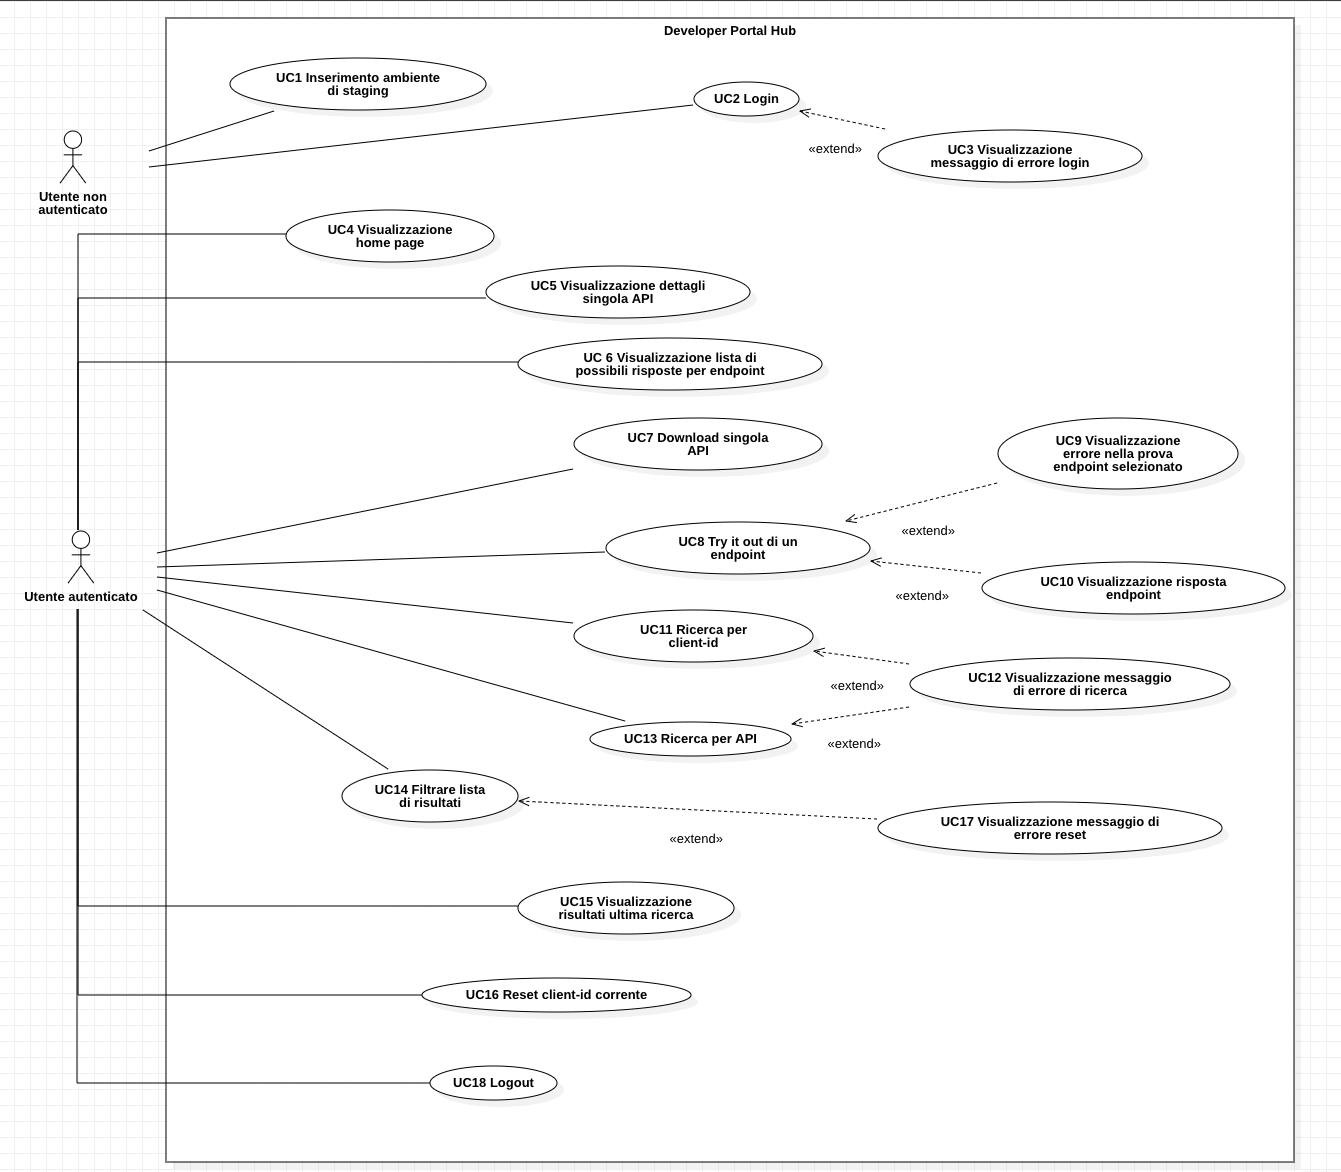
\includegraphics[width=0.9\columnwidth]{usecase/scenario-principale} 
    \caption{Use Case - UC0: Scenario principale}
\end{figure}

\begin{usecase}{0}{Scenario principale}
\usecaseactors{Sviluppatore applicativi}
\usecasepre{Lo sviluppatore è entrato nel plug-in di simulazione all'interno dell'IDE}
\usecasedesc{La finestra di simulazione mette a disposizione i comandi per configurare, registrare o eseguire un test}
\usecasepost{Il sistema è pronto per permettere una nuova interazione}
\label{uc:scenario-principale}
\end{usecase}

\section{Tracciamento dei requisiti}

Da un'attenta analisi dei requisiti e degli use case effettuata sul progetto è stata stilata la tabella che traccia i requisiti in rapporto agli use case.\\
Sono stati individuati diversi tipi di requisiti e si è quindi fatto utilizzo di un codice identificativo per distinguerli.\\
Il codice dei requisiti è così strutturato R(F/Q/V)(N/D/O) dove:
\begin{enumerate}
	\item[R =] requisito
    \item[F =] funzionale
    \item[Q =] qualitativo
    \item[V =] di vincolo
    \item[N =] obbligatorio (necessario)
    \item[D =] desiderabile
    \item[Z =] opzionale
\end{enumerate}
Nelle tabelle \ref{tab:requisiti-funzionali}, \ref{tab:requisiti-qualitativi} e \ref{tab:requisiti-vincolo} sono riassunti i requisiti e il loro tracciamento con gli use case delineati in fase di analisi.

\newpage

\begin{table}%
\caption{Tabella del tracciamento dei requisti funzionali}
\label{tab:requisiti-funzionali}
\begin{tabularx}{\textwidth}{lXl}
\hline\hline
\textbf{Requisito} & \textbf{Descrizione} & \textbf{Use Case}\\
\hline
RFN-1     & L'interfaccia permette di configurare il tipo di sonde del test & UC1 \\
\hline
\end{tabularx}
\end{table}%

\begin{table}%
\caption{Tabella del tracciamento dei requisiti qualitativi}
\label{tab:requisiti-qualitativi}
\begin{tabularx}{\textwidth}{lXl}
\hline\hline
\textbf{Requisito} & \textbf{Descrizione} & \textbf{Use Case}\\
\hline
RQD-1    & Le prestazioni del simulatore hardware deve garantire la giusta esecuzione dei test e non la generazione di falsi negativi & - \\
\hline
\end{tabularx}
\end{table}%

\begin{table}%
\caption{Tabella del tracciamento dei requisiti di vincolo}
\label{tab:requisiti-vincolo}
\begin{tabularx}{\textwidth}{lXl}
\hline\hline
\textbf{Requisito} & \textbf{Descrizione} & \textbf{Use Case}\\
\hline
RVO-1    & La libreria per l'esecuzione dei test automatici deve essere riutilizzabile & - \\
\hline
\end{tabularx}
\end{table}%

    \chapter{Progettazione e codifica}
\label{cap:progettazione-codifica}

\intro{Breve introduzione al capitolo}\\

\section{Tecnologie e strumenti}
\label{sec:tecnologie-strumenti}

Di seguito viene data una panoramica delle tecnologie e strumenti utilizzati.

\subsection*{Tecnologia 1}
Descrizione Tecnologia 1.

\subsection*{Tecnologia 2}
Descrizione Tecnologia 2

\section{Ciclo di vita del software}
\label{sec:ciclo-vita-software}

\section{Progettazione}
\label{sec:progettazione}

\subsubsection{Namespace 1} %**************************
Descrizione namespace 1.

\begin{namespacedesc}
    \classdesc{Classe 1}{Descrizione classe 1}
    \classdesc{Classe 2}{Descrizione classe 2}
\end{namespacedesc}


\section{Design Pattern utilizzati}

\section{Codifica}

    \chapter{Struttura principale e progettazione}\label{cap:struttura-progettazione}

\intro{In questo capitolo sono descritte la struttura principale del progetto e le attività di progettazione dell'applicativo.
Inoltre vengono descritte le tecnologie utilizzate durante lo sviluppo del progetto e le scelte architetturali.
}

\section{Tecnologie utilizzate}\label{sec:tecnologie-utilizzate}
Di seguito viene data una panoramica delle tecnologie utilizzate durante lo sviluppo del progetto di stage.

\subsection{Frontend}\label{subsec:frontend}
\subsubsection{Vue.js}\label{subsubsec:vue-js}
\textit{Vue.js} è un \textit{framework JavaScript} progressivo e reattivo, utilizzato per lo sviluppo di interfacce utente dinamiche e moderne. 
Creato da \textit{Evan You}, \textit{Vue.js} è apprezzato per la sua semplicità d'uso e flessibilità. Con un sistema di reattività basato su un modello di oggetti e dipendenze, 
\textit{Vue.js} rende facile il monitoraggio e l'aggiornamento automatico dell'interfaccia utente in base ai cambiamenti di stato dei dati. La sua architettura basata 
su componenti consente di organizzare il codice in moduli riutilizzabili e autonomi, semplificando la creazione di applicazioni complesse. 
Grazie alle direttive, è possibile arricchire il \glsfirstoccur{\gls{domg}} con funzionalità reattive, mentre il sistema di \textit{routing} agevola la creazione di \glsfirstoccur{\gls{spag}}. 
Con una crescita costante della comunità di sviluppatori, \textit{Vue.js} è diventato un'opzione popolare nel mondo dello sviluppo frontend.
Per il mio progetto ho utilizzato la versione 3 di \textit{Vue.js}, insieme allo \textit{script setup}, che è una nuova sintassi per definire componenti, progettata per semplificare la struttura del codice~\cite{site:vue.js}.

\subsubsection{TypeScript}\label{subsubsec:typeScript}
\textit{TypeScript} è un linguaggio di programmazione \glsfirstoccur{\gls{opensourceg}} sviluppato da \textit{Microsoft}. Si basa su \textit{JavaScript} e offre tipizzazione statica opzionale, 
consentendo agli sviluppatori di specificare tipi per variabili, parametri di funzioni e oggetti. Questa caratteristica aiuta a individuare errori e a migliorare 
la manutenibilità del codice~\cite{site:typescript}.\\
All'interno del mio progetto ho creato per la parte frontend una cartella chiamata \textit{types}, che contiene un file \textit{TypeScript} con al suo interno tutti i tipi utilizzati nel progetto.
\subsubsection{Vite.js}\label{subsubsec:vite}
\textit{Vite.js} è un \textit{build tool} utilizzato per lo sviluppo di applicazioni web. È stato creato da \textit{Evan You}, lo stesso creatore di \textit{Vue.js}, e si basa su \glsfirstoccur{\gls{rollupjsg}}.
\textit{Vite.js} è stato progettato per essere veloce, semplice da utilizzare e facile da configurare. La sua velocità è dovuta al fatto che utilizza la tecnica dell'\glsfirstoccur{\gls{esmg}} (\textit{ECMAScript Modules})
che permette di caricare i moduli in modo asincrono, riducendo i tempi di compilazione e di \glsfirstoccur{\gls{hotreloadg}}~\cite{site:vite}.
\subsubsection{Sass}\label{subsubsec:sass}
\textit{Sass} è un'estensione di \textit{CSS} che offre funzionalità aggiuntive e avanzate per semplificare e organizzare il modo in cui viene scritto e gestito il codice.
Può essere considerato un preprocessore \textit{CSS}, in quanto viene compilato in \textit{CSS} prima di essere interpretato dal \textit{browser}. \textit{Sass} inoltre permette di utilizzare funzionalità non disponibili in \textit{CSS} nativo, offrendo una serie di funzioni, variabili, \glsfirstoccur{\gls{mixing}} e altro~\cite{site:sass}.\\
Insieme a \textit{Sass}, ho utilizzato \textit{BEM}, ovvero una metodologia di \textit{naming convention} utilizzata nel mondo dello sviluppo web.

\subsection{Backend}\label{subsec:backend}
\subsubsection{Nest.js}\label{subsubsec:nest-js}
\textit{Nest.js} è un \textit{framework} per applicazioni \textit{server-side} basato su \textit{Node.js}. Si basa su \glsfirstoccur{\gls{expressjsg}} e \textit{TypeScript} ed è progettato per creare applicazioni scalabili e performanti.
Il \textit{framework} in questione combina concetti e caratteristiche provenienti da diversi paradigmi di sviluppo, tra cui la programmazione orientata agli oggetti (OOP), la programmazione funzionale e la programmazione reattiva~\cite{site:nest.js}.

\subsection{Altre tecnologie di supporto}\label{subsec:altre-tecnologie-di-supporto}
\subsubsection{Node.js}\label{subsubsec:node-js}
\textit{Node.js} è un ambiente di \textit{runtime JavaScript open-source} progettato per eseguire codice lato server~\cite{site:node}. Per gestire le dipendenze del mio progetto,
ho deciso di utilizzare \glsfirstoccur{\gls{pnpmg}} come gestore di pacchetti. Questa selezione ha portato a un miglior utilizzo delle risorse di sistema e ha notevolmente accelerato il processo di 
installazione delle dipendenze.
\subsubsection{Pinia}\label{subsubsec:pinia}
\textit{Pinia} è una libreria per la gestione dello stato per applicazioni \textit{Vue.js}. Promuove l'uso di \textit{store} modulari, ognuno dei quali gestisce uno stato specifico dell'applicazione~\cite{site:pinia}.
\subsubsection{Vue-router}\label{subsubsec:vue-router}
\textit{Vue-router} è una libreria per la gestione delle \textit{route} per le applicazioni \textit{Vue.js}. Permette di definire le \textit{route} dell'applicazione e di navigare tra le pagine~\cite{site:vue-router}.

\subsection{Versionamento}\label{subsec:versionamento}
\subsubsection{Git}\label{subsubsec:git}
\textit{Git} è un sistema di controllo versione distribuito e altamente flessibile, utile per tenere traccia delle modifiche apportate al codice sorgente durante lo sviluppo di un progetto \glsfirstoccur{\gls{softwareg}}~\cite{site:git}.
\subsubsection{CodeCommit}\label{subsubsec:code-commit}
\textit{AWS CodeCommit} rappresenta un servizio di \textit{hosting} di \textit{repository} altamente scalabile, che è gestito all'interno dell'ecosistema di \glsfirstoccur{\gls{awsg}} (\textit{Amazon Web Services}). 
Con \textit{CodeCommit}, è possibile ospitare \textit{repository Git} privati in un ambiente sicuro e flessibile~\cite{site:code-commit}.

\subsection{Verifica}\label{subsec:verifica}
\subsubsection{ESLint}\label{subsubsec:eslint}
\textit{ESLint} è uno strumento \textit{open-source} ampiamente utilizzato per l'analisi statica del codice \textit{JavaScript}. Esso permette di identificare e segnalare potenziali errori o pratiche non conformi durante la fase di sviluppo.
\subsubsection{Vitest}\label{subsubsec:vitest}
\textit{Vitest} è un \textit{framework} per l'implementazione di test di unità, utilizzato prevalentemente in progetti \textit{Vue.js}.
Usato in coppia con \textit{Vite} permette di eseguire test di unità in modo più veloce e semplice~\cite{site:vitest}.

\subsection{Librerie esterne utilizzate}\label{subsec:librerie-esterne}
\subsubsection{THRON Components}\label{subsubsec:thron-components}
La libreria \textit{THRON Components} contiene i componenti utilizzati per creare elementi comuni, come i bottoni del portale, seguendo il \textit{design system} aziendale.
\subsubsection{Azure MSAL}\label{subsubsec:azure-MSAL}
\textit{Azure MSAL} è una libreria che permette di integrare il login con \glsfirstoccur{\gls{azureadg}} (\textit{Azure Active Directory}) all'interno di un'applicazione web~\cite{site:msal}.
\subsubsection{Swagger UI}\label{subsubsec:swagger-ui}
\textit{Swagger UI} è una libreria \textit{open-source} progettata per semplificare la visualizzazione e l'interazione con la documentazione delle \textit{API}~\cite{site:swagger}.

\section{Struttura principale del sistema}\label{sec:struttura-principale-sistema}
Il sistema è composto da due principali sezioni:
\begin{itemize}
  \item Frontend, ovvero l'interfaccia utente dell'applicazione web che permette all'utilizzatore di interagire con il sistema. È responsabile di presentare i contenuti in modo visivamente attraente e interattivo, consentendo agli utenti di navigare, inserire dati e svolgere azioni specifiche. Per lo
  sviluppo di questa parte del sistema è stato utilizzato il \textit{framework Vue.js};
  \item Backend, ovvero la parte del sistema che elabora le richieste provenienti dal frontend e restituisce i risultati. È responsabile della gestione dei dati e della logica di \textit{business}.
  Lo sviluppo di questa parte del sistema è stato realizzato utilizzando il \textit{framework Nest.js}. 
\end{itemize}

\subsection{Ambienti di sviluppo}\label{subsec:ambienti-sviluppo}
Gli ambienti di \textit{staging} sono ambienti di test che vengono utilizzati per testare le funzionalità dell'applicazione prima di rilasciarla in produzione.
A livello aziendale sono stati definiti tre ambienti di cui i primi due di \textit{staging}, denominati come segue:
\begin{itemize}
  \item \textbf{\textit{Development}}: consente di validare a livello tecnico le funzionalità;
  \item \textbf{\textit{Quality}}: consente di validare a livello funzionale o di implementazione le funzionalità;
  \item \textbf{\textit{Production}}: ambiente di produzione in cui viene rilasciata la funzionalità.
\end{itemize}

\subsection{Configurazione dell'ambiente per lo sviluppo del progetto}\label{subsec:configurazione-ambiente-sviluppo}
Il progetto di stage, necessita di cartelle per la configurazione dell'ambiente di sviluppo, per la configurazione del progetto e per la configurazione del \textit{deploy}.
Più precisamente, il progetto segue la seguente struttura:

\subsubsection*{\emph{Buildspec}}\label{subsubsec:buildspec}
La cartella \textit{Buildspec} contiene i file di configurazione per la \textit{build} dell'applicazione su \glsfirstoccur{\gls{awscodebuildg}}.
Questo è il primo step del processo di \textit{deploy}, in quanto viene eseguita la \textit{build} sia del \textit{middleware} che del portale.
La cartella è formata a sua volta da tre file: \textit{buildspec\_development}, \textit{buildspec\_quality} e \textit{buildspec\_production}. 
Ognuno di questi file configura la \textit{build} dell'applicazione in base all'ambiente di \textit{deploy}.\\
Successivamente dopo aver effettuato tutti i comandi specificati nei file \textit{buildspec}, inizia lo step di \textit{deploy}, specificato nella cartella \textit{Infra}.
Ognuno dei file \textit{buildspec} è un file \textit{YAML}, che è formato dalle seguenti sezioni:
\begin{itemize}
  \item La sezione \textit{env} dove vengono specificate le variabili d'ambiente utilizzate nel progetto;
  \item La sezione di \textit{pre-build} dove vengono specificati i comandi da eseguire prima della \textit{build};
  \item La sezione di \textit{build} dove vengono specificati i comandi per la \textit{build} del portale e del \textit{middleware}.
\end{itemize}

\subsubsection*{\emph{Infra}}\label{subsubsec:infra}
La cartella \textit{Infra} contiene i file di configurazione per il \textit{deploy} dell'applicazione su \textit{AWS}. È scritta utilizzando il linguaggio di programmazione \glsfirstoccur{\gls{pythong}}.\\
La cartella è formata da due file: `\textit{app.py}' e `\textit{stack.py}'. Il primo file contiene la configurazione per il \textit{deploy} dell'applicazione, mentre il secondo file contiene la configurazione per il \textit{deploy} dell'infrastruttura.\\
Per quanto riguarda l'infrastruttura del progetto, ho utilizzato e configurato due costrutti, anche chiamati \textit{CDK Constructs} o semplicemente \textit{Constructs}, che sono delle classi che rappresentano un componente dell'infrastruttura.
Il primo costrutto si chiama \textit{THRONCloudFrontDistribution} e consente di accelerare la distribuzione dei contenuti web statici e dinamici, come file \textit{HTML}, \textit{CSS}, \textit{JS} e immagini, agli utenti.
In breve questo costrutto genera il \textit{template} di \glsfirstoccur{\gls{awscloudfrontg}} ed esegue il \textit{deploy} degli \textit{asset} statici su un \glsfirstoccur{\gls{s3g}}.\\
Il secondo costrutto che ho utilizzato si chiama \textit{THRONDockerLambda} e consente di creare una funzione \glsfirstoccur{\gls{lambdag}} in cui il gestore è un'immagine \glsfirstoccur{\gls{dockerg}}.
Nel caso del mio progetto, mi è servito per creare una \textit{lambda} che una volta invocata avvia un \textit{docker} con all'interno il progetto backend.\\

\subsubsection*{\emph{Middleware}}\label{subsubsec:middleware}
La cartella \textit{Middleware} contiene il progetto backend in \textit{Nest.js}. Nello specifico la cartella è formata dalle seguenti sezioni:
\begin{itemize}
  \item La cartella \textit{src} che contiene il codice sorgente dell'applicazione, dove vengono specificati i vari \textit{endpoint} che utilizzo sulla parte frontend, lo \textit{script} per la configurazione
  della \textit{lambda}, una cartella con gli \textit{helpers} e la cartella del \textit{middleware};
  % \item La cartella test che contiene i test di unità dell'applicazione;
  \item File \textit{env} che contiene le variabili d'ambiente utilizzate nel progetto;
  \item Una cartella \textit{node\_modules} che contiene le dipendenze del progetto.
\end{itemize}
\subsubsection*{\emph{Portal}}\label{subsubsec:portal}
La cartella \textit{portal} contiene il progetto frontend in \textit{Vue.js}. Nello specifico la cartella è formata dalle seguenti sezioni:
\begin{itemize}
  \item La cartella \textit{public} contenente il file `\textit{index.html}', ovvero il file principale dell'applicazione;
  \item Una cartella \textit{node\_modules} che contiene le dipendenze del progetto;
  \item La cartella \textit{src} che contiene il codice sorgente dell'applicazione, dove vengono specificati i vari componenti che utilizzo, i vari \textit{store}, i vari \textit{router} e le varie \textit{utilities};
  \item File \textit{env} che contiene le variabili d'ambiente utilizzate nel progetto.
\end{itemize}

\subsubsection*{\emph{Dockerfile}}\label{subsubsec:dockerfile}
Il file \textit{Dockerfile} è un file \textit{docker} che contiene le istruzioni per creare un'immagine che viene utilizzata per eseguire il \textit{middleware} all'interno di una \textit{lambda}.\\
Utilizzando la struttura \textit{Dockerfile}, ho creato un ambiente isolato in cui il \textit{middleware} può essere configurato e utilizzato come parte della mia funzione 
\textit{lambda}. Quando la funzione viene invocata, avvia il \textit{Docker} \glsfirstoccur{\gls{containerg}} ed esegue il \textit{middleware} all'interno dell'ambiente containerizzato, 
garantendo che esso sia parte integrante dell'applicazione \glsfirstoccur{\gls{serverlessg}}.

\section{Progettazione}\label{sec:progettazione}

\subsection{Architettura frontend}\label{subsec:architettura-front-end}
\subsubsection{Architettura Vue.js}\label{subsubsec:architettura-vue-js}
\textit{Vue.js} è un \textit{framework} utilizzato nelle \textit{single page applications}, che permette di definire le pagine web in modo modulare, utilizzando componenti riutilizzabili.
I componenti costituiscono la base dell'architettura di \textit{Vue}. Essi rappresentano una parte isolata dell'interfaccia, che può contenere il proprio modello, i propri stili e la propria logica, infatti ogni componente ha il proprio
\textit{template} scritto in \textit{HTML}, il proprio \textit{script} scritto nel mio caso in \textit{TypeScript} e i propri stili scritti nel mio caso in \textit{Scss}.
Come già accennato in precedenza, i componenti sono riutilizzabili all'interno di un'applicazione e possono essere combinati tra loro per creare gerarchie di interfacce ancora più complesse.\\

L'architettura di \textit{Vue.js} è basata sul pattern architetturale \textit{MVVM} (\textit{Model-View-ViewModel}), che è una variante del pattern \glsfirstoccur{\gls{mvcg}} (\textit{Model-View-Controller}), dove:
\begin{itemize}
  \item \textbf{\textit{Model}}: rappresenta lo stato, i dati e le regole di \textit{business} dell'applicazione, che gestiscono l'accesso e la modifica di tali dati. Lo stato viene definito tramite l'uso
  di particolari variabili di tipo reattivo, che permettono di aggiornare automaticamente la \textit{View} associata in caso di modifiche;
  \item \textbf{\textit{View}}: è l'interfaccia utente, che visualizza i dati contenuti nel \textit{Model} e si occupa di reagire agli input dell'utente. La \textit{View} è definita utilizzando i template \textit{Vue.js} e viene reattivamente aggiornata in base ai cambiamenti del modello. La vista viene definita utilizzando un \textit{template}, ovvero una direttiva dell'\textit{HTML}, arricchita con alcune direttive \textit{Vue.js}. 
  Queste particolari direttive permettono di collegare elementi del \textit{DOM} a proprietà o metodi del modello, in modo che la \textit{View} possa reagire agli input dell'utente e aggiornare automaticamente lo stato dell'applicazione;
  \item \textbf{\textit{ViewModel}}: è l'intermediario tra la \textit{View} e il \textit{Model}. Il \textit{ViewModel} gestisce la logica dell'interfaccia utente e mantiene lo stato dell'applicazione sincronizzato con la \textit{View}.
  Il \textit{ViewModel} è rappresentato da un componente \textit{Vue.js}, infatti esso è un'istanza che collega il modello e la vista. All'interno di un componente è possibile definire metodi, proprietà 
  computate, metodi del ciclo di vita, gestione di eventi e molte altre funzionalità. Questo consente di definire la logica di presentazione e di manipolare i dati all'interno di un contesto definito.
\end{itemize}

In breve, l'architettura è incentrata sulla creazione e utilizzo di componenti riutilizzabili che al loro interno incorporano sia il modello che la vista. Un aspetto che rende \textit{Vue.js}
diverso da altri \textit{framework} è proprio il concetto di reattività, infatti \textit{Vue.js} è in grado di rilevare automaticamente le dipendenze tra i componenti, in modo da poter aggiornare automaticamente l'interfaccia utente~\cite{site:vue-architettura}.

\subsection{Architettura backend}\label{subsec:architettura-backend}
\subsubsection{Architettura Nest.js}\label{subsubsec:architettura-nest-js}
L'architettura di \textit{Nest.js} si basa su diversi principi chiave e concetti fondamentali che lo rendono un \textit{framework} efficace per la creazione di applicazioni \textit{server-side}.
La caratteristica principale di \textit{Nest.js} è la modularità, che promuove la suddivisione dell'applicazione in moduli, consentendo di organizzare il codice in unità funzionali e riutilizzabili.\\
Di seguito i concetti base su cui si basa l'architettura:
\begin{itemize}
  \item \textbf{\textit{Module}}: rappresenta un'unità organizzativa dell'applicazione che contiene un gruppo di elementi correlati come \textit{Controller}, \textit{Service} e \textit{Provider}. Questa struttura modulare 
  favorisce la separazione delle responsabilità rendendo il codice più leggibile;
  \item \textbf{\textit{Controller}}: sono interfacce tra la rete e la logica dell'applicazione responsabili della gestione delle richieste \glsfirstoccur{\gls{httpg}} in ingresso. Ogni \textit{Controller} è associato a un percorso specifico e a uno o più metodi che rappresentano le diverse azioni eseguibili sul percorso;
  \item \textbf{\textit{Service}}: contiene la logica di \textit{business} dell'applicazione. I \textit{Service} si occupano della gestione dei dati e dell'interazione con le risorse esterne~\cite{site:nest-architettura}.
\end{itemize}

    \chapter{Conclusioni}
\label{cap:conclusioni}

\section{Consuntivo finale}

\section{Raggiungimento degli obiettivi}

\section{Conoscenze acquisite}

\section{Valutazione personale}


    \appendix
    \chapter{Appendice A}

\epigraph{Citazione}{Autore della citazione}


    \backmatter
    \printglossary[type=\acronymtype, title=Acronimi e abbreviazioni, toctitle=Acronimi e abbreviazioni]
    \printglossary[type=main, title=Glossario, toctitle=Glossario]

    \cleardoublepage
\chapter{Bibliografia}

\nocite{*}

% Print book bibliography
\printbibliography[heading=subbibliography,title={Riferimenti bibliografici},type=book]

% Print site bibliography
\printbibliography[heading=subbibliography,title={Siti web consultati},type=online]

\end{document}
